\chapter{Konfliktbehandlung}
\label{Konfliktbehandlung}

Bei der gemeinsamen Bearbeitung von Dokumenten mit PouchDB zwischen mehreren Clients kann es unter bestimmten Umständen zu Konflikten kommen \cite{pouch:conflicts}. Allerdings kommt es auf das verwendete Datenmodell und die Anwendungsarchitektur an, ob und wie häufig Konflikte auftreten.

\section{Auftreten von Konflikten}

PouchDB unterscheidet zwischen zwei Arten von Konflikten: Den \emph{immediate conflicts} (sofortige Konflikte) und den \emph{eventual conflicts} (irgendwann auftretende Konflikte). 

\emph{Immediate conflicts} können bei der Synchronisation zwischen Client und Server auftreten und können durch ein erneutes \texttt{put()} aufgelöst werden \cite{pouch:conflicts}.

\emph{Eventual conflicts} sind Konflikte, die aus einer gleichzeitigen Änderung eines Dokuments durch mehrere Clients resultieren. In einer Anwendung, die nur das Neuanlegen bzw. Löschen vorhandener Dokumente erlaubt, können somit keine \emph{eventual conflicts} auftreten. \emph{Eventual conflicts} treten bei der Verwendung von PouchDB nicht sofort beim Schreibzugriff auf. Erst die CouchDB-Instanz, zu der synchronisiert wird, bemerkt den Konflikt und bestimmt sofort einen Gewinner aus beiden Revisionen. Die Verlierer-Revision wird nicht gelöscht, sondern unter einer anderen Revisions-Id gespeichert. Dies erlaubt eine spätere Konfliktbehandlung \cite{pouch:conflicts}.

\section{Konflikte in PouchDB}

PouchDB behandelt Konflikte mit einer Baumstruktur, die an das Branch-System von Git angelehnt ist \cite{pouch:conflicts}. 

Dabei kann der Client alle konfliktierenden Revisionen eines Dokuments erhalten, indem beim Laden der Dokumente die Option \mbox{\texttt{\{conflicts: true\}}} angegeben wird. Sind bei einem Dokument Konflikte vorhanden, finden sich diese anschließend im Feld \texttt{\_conflicts} des JSON-Dokuments, wie das folgende Listing zeigt:

\begin{codebox}
	\begin{lstlisting}[style=typescript]
{
	"_id": "docid",
	"_rev": "2-x",
	"_conflicts": ["2-y"]
}
	\end{lstlisting}
\end{codebox}

Das so erhaltene Dokument stellt den zeitweiligen Gewinner der Konfliktbehandlung von CouchDB dar.
Das Feld \texttt{\_conflicts} stellt ein String-Array dar, das die verschiedenen Verlierer-Revisionen des Dokuments referenziert. Diese Revisionen können zum Vergleich einzeln geladen werden.

Zur Konfliktbehandlung mit PouchDB muss das Dokument, das vom Benutzer oder Entwickler als Gewinner ausgewählt wird, als neue Revision über dem zeitweiligen Gewinner mit einem \texttt{put()} eingefügt werden. Anschließend müssen die anderen konfliktierenden Revisionen gelöscht werden.

\section{Umsetzung der Konfliktauflösung in der Demo-Anwendung}

Zur Beispielhaften Umsetzung der Konfliktauflösung mit PouchDB in der Demo-Anwendung wurden zwei Ansätze gewählt: Ein \emph{Last Wins}-Konzept, bei der die letzte Änderung am Dokument als Gewinner ausgewählt wird sowie ein \emph{Merge}-Konzept, bei dem alle konfliktierenden Revisionen zu einem neuen Dokument zusammengeführt werden.

Um die Varianten der Konfliktbehandlung möglichst dynamisch austauschen zu können, wurden diese in der Demo-Anwendung als Strategie-Muster implementiert.

\begin{figure}[htb]
	\centering
	\caption{Klassendiagramm: Strategie-Muster für Konfliktauflösung}
	\label{fig:conflictresolutionstrategy}
	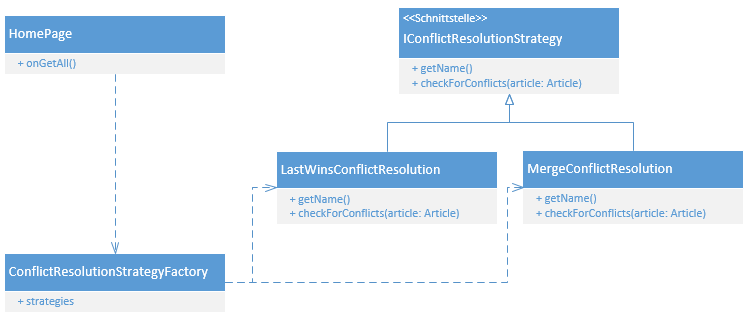
\includegraphics[width=\textwidth]{\figdir/ConflictResolution.png}
\end{figure}

Abbildung \ref{fig:conflictresolutionstrategy} zeigt das verwendete Strategie-Muster. Beide Strategien implementieren das Interface \texttt{IConflictResolutionStrategy}, das die Methoden \texttt{getName()} (für die Auswahl in der Oberfläche) und \texttt{checkForConflicts(article: Article)} (zur eigentlichen Konfliktauflösung) vorschreibt.

Eine Factory (\texttt{ConflictResolutionStrategyFactory}) bekommt beide Strategien per \emph{Dependency Injection} übergeben und kann diese anschließend an die Klasse HomePage übergeben, wo beide Strategien ausgewählt und verwendet werden können.